%    Documentation for PRU ADC Project
%    Copyright (C) 2016  Gregory Raven
%
%    This program is free software: you can redistribute it and/or modify
%    it under the terms of the GNU General Public License as published by
%    the Free Software Foundation, either version 3 of the License, or
%    (at your option) any later version.
%
%    This program is distributed in the hope that it will be useful,
%    but WITHOUT ANY WARRANTY; without even the implied warranty of
%    MERCHANTABILITY or FITNESS FOR A PARTICULAR PURPOSE.  See the
%    GNU General Public License for more details.
%
%    You should have received a copy of the GNU General Public License
%    along with this program.  If not, see <http://www.gnu.org/licenses/>.

\documentclass[oneside,letterpaper,12pt]{book}
\usepackage[utf8]{inputenc}
\usepackage[T1]{fontenc}
\usepackage[top=0.8874in,bottom=0.8874in,left=0.7874in,right=0.7874in]{geometry}
\usepackage{charter}
\usepackage{color}
\usepackage{array,ragged2e}
\usepackage{graphicx}
\usepackage[colorlinks=true, linkcolor=red]{hyperref}
\usepackage{amsmath}
\usepackage{titling,lipsum}
\usepackage{booktabs}
\usepackage{longtable}
\usepackage{float}
\usepackage{parskip}


\title{This is title of my document}

\begin{document}
%    Documentation for Irrigation Control Project
%    Copyright (C) 2017  Gregory Raven
%
%    This program is free software: you can redistribute it and/or modify
%    it under the terms of the GNU General Public License as published by
%    the Free Software Foundation, either version 3 of the License, or
%    (at your option) any later version.
%
%    This program is distributed in the hope that it will be useful,
%    but WITHOUT ANY WARRANTY; without even the implied warranty of
%    MERCHANTABILITY or FITNESS FOR A PARTICULAR PURPOSE.  See the
%    GNU General Public License for more details.
%
%    You should have received a copy of the GNU General Public License
%    along with this program.  If not, see <http://www.gnu.org/licenses/>.

\thispagestyle{empty}
{\centering\bfseries\color{black}\Huge
Irrigation Controller Using Beaglebone Green Wireless, Node.js, and Ecmascript 6
\par}

\bigskip

\begin{figure}
	\centering
	\includegraphics[width=\textwidth]{photos/cover_photo}
\end{figure}

\bigskip
{\centering\bfseries\Large
Gregory Raven
\par}


\bigskip
{\centering\bfseries\LARGE
June 13, 2017
\par}
%\newpage





%\setcounter{page}{1}

%\author{Gregory Raven}
%\title{Using the Beaglebone Black Programmable Real-Time Unit with the RemoteProc and Remote Messaging Framework to Capture and Play Data from an ADC}
%\date{October 2016}

%
\frontmatter
Beaglebone Green PRU PID Motor Speed Control Project

Copyright 2016 by Gregory Raven

Some content is based on material published by Texas Instruments.
Please see the TI license agreement included in the Github repository.
%\maketitle
\tableofcontents
\listoftables
\listoffigures
%\maketitle

\mainmatter
%    Documentation for PRU ADC Project
%    Copyright (C) 2016  Gregory Raven
%
%    This program is free software: you can redistribute it and/or modify
%    it under the terms of the GNU General Public License as published by
%    the Free Software Foundation, either version 3 of the License, or
%    (at your option) any later version.
%
%    This program is distributed in the hope that it will be useful,
%    but WITHOUT ANY WARRANTY; without even the implied warranty of
%    MERCHANTABILITY or FITNESS FOR A PARTICULAR PURPOSE.  See the
%    GNU General Public License for more details.
%
%    You should have received a copy of the GNU General Public License
%    along with this program.  If not, see <http://www.gnu.org/licenses/>.

\chapter{Introduction}

This is the documentation for an embedded GNU/Linux project utilizing the RemoteProc and RPMsg framework in the Beaglebone Green (BBG) development board.  The project repository is located here:

\url{https://github.com/Greg-R/pru-pid-motor}

The inspiration for this project came from an example project published by Texas Instruments.  The Texas Instruments project is based on "Code Composer Studio", which is an "Integrated Development Environment" (IDE):

\url{http://processors.wiki.ti.com/index.php/PRU_Training:_PRU_PID_Motor_Demo}

There is also a PDF file which describes the project in detail:

\url{http://www.ti.com/lit/ug/tidubj6/tidubj6.pdf}

The TI project requires a relatively complex cross-compiler installation.  This project is designed to be done via SSH terminal connection, and all software compilation was done on the Beaglebone Green target device using the PRU C compiler (clpru).  The VIM text editor was used to edit files, however, any text editor available in the Debian distribution can be used.

The Debian-based GNU/Linux distribution used on the BBG can be downloaded from this page:

\url{http://beagleboard.org/latest-images}

The ``IOT'' (non-GUI) image was chosen, as this provides the shortest path to get the project up and running.

Recent developments in the Texas Instruments PRU support include the RemoteProc and Remote Messaging frameworks, as well as an extensively documented C compiler and much additional supporting documentation.  This project utilizes these frameworks and is entirely dependent upon C code in both the PRU and GNU/Linux user space.  For further information, refer to the detailed examples provided by TI in the ``PRU Support Package'':

\url{https://git.ti.com/pru-software-support-package}

A listing of additional resources is found in the Resources chapter.

The motor recommended by TI was purchased and tested.  However, a better motor with an integrated quadrature encoder was found on eBay and is recommended.  A chapter is included which describes this motor-encoder and how to obtain one.

\section{Project Goals}

This project demonstrates an electronic speed control for a DC motor which is implemented with the PRUs included with the Beaglebone Green.  Beyond its usefulness as a demonstration project, it could be used in a robotics project such as a ``mobile robot''.

The basic principle of the speed controller is "Proportional Integral Derivative" (PID) feedback control, which is a common feedback controller used in digital systems.

Here is an excellent reference article on PID controllers:

\url{http://www.wescottdesign.com/articles/pid/pidWithoutAPhd.pdf}

\section{Limitations}

All of the development was done as root user via ssh on the BeagleBone Green.  This is generally not a good practice, however, considering this as an embedded and experimental project it was not considered to be a serious drawback.

No attempt was made to optimize the response of the PID controller.  The default values for the PID controller create a stable loop with the recommended DC motor-encoder.  Optimization will depend on the particular motor-encoder chosen and this task is left to the interested experimenter.



%    Documentation for PRU ADC Project
%    Copyright (C) 2016  Gregory Raven
%
%    This program is free software: you can redistribute it and/or modify
%    it under the terms of the GNU General Public License as published by
%    the Free Software Foundation, either version 3 of the License, or
%    (at your option) any later version.
%
%    This program is distributed in the hope that it will be useful,
%    but WITHOUT ANY WARRANTY; without even the implied warranty of
%    MERCHANTABILITY or FITNESS FOR A PARTICULAR PURPOSE.  See the
%    GNU General Public License for more details.
%
%    You should have received a copy of the GNU General Public License
%    along with this program.  If not, see <http://www.gnu.org/licenses/>.

\chapter{System Diagrams}

\begin{figure}[H]
	\centering
	\includegraphics[width=0.6\textwidth]{diagrams/system_diagram}
	\centering\bfseries
	\caption{Beagle Bone Green Wireless Irrigation Control System}
\end{figure}

The above diagram shows the main components of the system.  A reference section 
is included which has a complete parts list.


\section{GNU/Linux Operating System on Host ARM Processor}

The command uname -a on the BBG used to develop this project reports this:

\begin{verbatim}
Linux BBG2 4.4.30-ti-r64 #1 SMP Fri Nov 4 21:23:33 UTC 2016 armv7l GNU/Linux
\end{verbatim}

The latest IOT image has a newer kernel.  It is not a major update as of December 18, 2016.







%    Documentation for PRU ADC Project
%    Copyright (C) 2016  Gregory Raven
%
%    This program is free software: you can redistribute it and/or modify
%    it under the terms of the GNU General Public License as published by
%    the Free Software Foundation, either version 3 of the License, or
%    (at your option) any later version.
%
%    This program is distributed in the hope that it will be useful,
%    but WITHOUT ANY WARRANTY; without even the implied warranty of
%    MERCHANTABILITY or FITNESS FOR A PARTICULAR PURPOSE.  See the
%    GNU General Public License for more details.
%
%    You should have received a copy of the GNU General Public License
%    along with this program.  If not, see <http://www.gnu.org/licenses/>.

\chapter{Ecmascript 6}

The following describes the simplest possible set-up.  Everything was done via the command line, and the vim editor was used extensively to develop the C code and shell scripts.

SSH was used to remotely access the BBG from a 64 bit desktop computer running Ubuntu 16.04.

For reference, here is the link to the TI PRU support package:

\url{https://git.ti.com/pru-software-support-package}

The above package can be cloned to the BBG.  There is a good set of examples and labs included.  The labs are documented here:

\url{http://processors.wiki.ti.com/index.php/PRU_Training:_Hands-on_Labs}

Note that the files appropriate for the BBG are in the folders with name am335x.

The Makefiles in the labs and examples were designed to work with a particular set-up which can be easily implemented on the BBG.

The following is a list of recommended steps to prepare a BBG for compiling PRU C files.
This process assumes a recent SD card image (IOT recommended) which is loaded with the PRU compiler (clpru) and libraries.  Another assumption is that the RemoteProc and RPMsg kernel drivers are included and that they are loaded during the start-up process.  This is true for some, but not all, recently published images as of December, 2016.

\section{Activate RemoteProc PRU and Kernel Modules}

The newest Beaglebone Debian distributions do not have the Remoteproc framework activated by default!

The following process activates the framework which includes several loadable kernel modules.  This is a prerequisite for the remainder of the setup process.

This process was tested using this image:

bone-debian-8.6-iot-armhf-2016-10-30-4gb.img

The ``IOT'' (Internet Of Things) image includes the set of tools required to install and compile the required software.
The image was found at this web site:

\url{http://elinux.org/Beagleboard:BeagleBoneBlack_Debian#microSD.2FStandalone:_.28iot.29_.28BeagleBone.2FBeagleBone_Black.2FBeagleBone_Green.29}

The IOT distribution includes very useful scripts in the following directory:

/opt/scripts/tools

The script grow\_partition.sh will expand the file system on the micro-sd card to its full capacity.  Running this script is highly recommended before proceeding with this process!

\section{Activate Remoteproc: Step-by-step Process}

\begin{enumerate}
\item  Write Beaglebone image to micro-sd and expand partition as required.
\item  Insert micro-sd into BBG slot, press boot and power buttons and release.  Non-flasher images may not require the boot button to be pressed, and the board will boot and run from the micro-sd card automatically.
\item  ssh debian@192.168.1.7 (or whatever the IP is set to).  If you are using a router with a GUI control application, it may have a display which indicates the board is connected and to which IP address has been assigned to it.
\item  Execute
\begin{verbatim}
sudo apt-get update
\end{verbatim}
\item  Execute
\begin{verbatim}
uname -r
\end{verbatim} 
to verify kernel version.  Please note that the RemoteProc framework is still evolving and it is recommended to verify that the kernel used will work with the PRU support package examples.

The rest of the set-up will be completed using root access.
Execute
\begin{verbatim}
sudo su
\end{verbatim}
and authenticate if required to switch to root user.
\item Clone this repository to a convenient directory (recommended /opt/scripts/tools):

\begin{verbatim}
git clone https://github.com/RobertCNelson/dtb-rebuilder
\end{verbatim}

\item Execute:
\begin{verbatim}
cd dtb-rebuilder/ 
cd src/arm
\end{verbatim}
\item Find and edit the top of the device tree dts file.
For BBG, this is:
\begin{verbatim}
am335x-bonegreen.dts
\end{verbatim}
Uncomment this single line in the file:
\begin{verbatim}
/*   #include "am33xx-pruss-rproc.dtsi"  */
\end{verbatim}

The line should now look like this:
\begin{verbatim}
#include "am33xx-pruss-rproc.dtsi"
\end{verbatim}

A new include statement must be added to the same file for configuration of the Quadrature Decoder and the PRU PWM.  This file must be copied from the repository:

\begin{verbatim}
pru-pid-motor/software/dtsi/am335x-boneblack-prupid.dtsi
\end{verbatim}

into the arm directory in the dtb-rebuilder.

Add this line to the end of the am335x-bonegreen.dts file:

\begin{verbatim}
#include "am335x-boneblack-prupid.dtsi"
\end{verbatim}
 
Save and exit.
\item
Execute:
\begin{verbatim}
cd /etc/modprobe.d
\end{verbatim}
Create a new file named:
\begin{verbatim}
pruss-blacklist.conf
\end{verbatim}
Note that the latest images may already have this file.

Add this single line to the file:
\begin{verbatim}
blacklist uio_pruss
\end{verbatim}
Save and exit.
\item
cd back to the dtb-rebuilder directory.  Execute these commands:
\begin{verbatim}
make 
make install 
reboot
\end{verbatim} 
\end{enumerate}
To verify that the above process was successful:

\begin{verbatim}
cd /sys/bus/platform/devices
ls
\end{verbatim}

Now look for the following in the output from the ls command:
\begin{verbatim}
4a300000.pruss
4a320000.intc
4a334000.pru0
4a338000.pru1
\end{verbatim}

The appearance of the above entries indicates that the RemoteProc PRU activation process was successful.

\section{PRU Compiler Setup Process}

\begin{enumerate}
\item  Execute these commands:
\begin{verbatim}
cd /
\end{verbatim} and then 
\begin{verbatim}
find . -name cgt-pru
\end{verbatim}

The path should be something like 
\begin{verbatim}
/usr/share/ti/cgt-pru
\end{verbatim}  

This is the location of the PRU library and includes.
However, the clpru compiler binary is not located in this directory.  Run this command:
\begin{verbatim}
which clpru
\end{verbatim}
and the result will be something like:
\begin{verbatim}
/usr/bin/clpru
\end{verbatim}
This is the path to the compiler binary.

The PRU C compiler needs to find the include and lib directories.  The Makefiles in the PRU Support Package look for the compiler binary at this path, so the following changes must be made.

Execute the following commands (as root):
\begin{verbatim}
cd /usr/share/ti/cgt-pru
mkdir bin
cd bin
ln -s /usr/bin/clpru clpru
\end{verbatim}
So now the Makefiles will find the compiler executable in the correct location via the link.
\item  Now install the PRU Support Package in the home directory:

\begin{verbatim}
cd /home/debian
git clone git://git.ti.com/pru-software-support-package/pru-software-support-package.git
\end{verbatim}

This will clone a copy of the latest pru support package.
\item  cd into lab\_5 in the package and execute the make command:
\begin{verbatim}
cd pru-software-support-package/labs/lab_5/solution/PRU_Halt
make
\end{verbatim}
This will fail, as the Makefile is looking for environment variable \$PRU\_CGT.  Execute:

\begin{verbatim}
export PRU_CGT=/usr/share/ti/cgt-pru
\end{verbatim}

Now execute the make command again.  It should succeed.  A new directory ``gen'' should appear.  The above command is included in the file ``pru\_gpio\_config'' in the shell\_scripts directory of the project's Github repository.

\item  Execute the following:
\begin{verbatim}
cd gen
cp PRU_Halt.out am335x-pru0-fw
cp am335x-pru0-fw /lib/firmware
\end{verbatim}
This renames the executable binary and copies it to the directory at which Remoteproc expects to find PRU firmwares.
\item  Now cd into the PRU\_RPMsg\_Echo\_Interrupt1 directory in the same lab\_5.
Edit main.c as follows:
\begin{verbatim}
//#define CHAN_NAME					"rpmsg-client-sample"
#define CHAN_NAME					"rpmsg-pru"
\end{verbatim}
The ``CHAN\_NAME'' define is now set to ``rpmsg-pru''.
\item  Now execute almost the same as \#9, except this time the firmware for PRU1 is compiled a copied:
\begin{verbatim}
make
cd gen
cp PRU_RPMsg_Echo_Interrupt1.out am335x-pru1-fw
cp am335x-pru1-fw /lib/firmware
\end{verbatim}
The compilation of both PRU firmwares are complete and they are copied to /lib/firmware.
\item  reboot
\item  Execute:

\begin{verbatim}
lsmod
\end{verbatim}

These kernel modules should be present in the output:

\begin{verbatim}
pru_rproc              15431  0 
pruss_intc              8603  1 pru_rproc
pruss                  12026  1 pru_rproc
\end{verbatim}
Now execute:
\begin{verbatim}
rmmod pru_rproc
modprobe pru_rproc
\end{verbatim}

The rmmod command removes the remoteproc module pru\_rproc.
The modprobe command re-inserts the same module.
\item  
\begin{verbatim}
cd /dev
ls
\end{verbatim} 

Look for rpmsg\_pru31 character device file.  It will be there!
This confirms that the PRU C compiler are properly configured and that the Makefile for this project will compile the PRU binaries successfully.  The RemoteProc drivers are also tested with the successful completion of the above set-up process.  This is not the entire configuration, however.
\end{enumerate}

\section{Additional Configuration Required to Compile the PRU Remoteproc Project}

Some components of the PRU Support Package need to be added to the PRU C compiler directories.  The Makefile expects to find these components in these directories.

Execute these commands in the directory in which the PRU Support Package was cloned:

\begin{verbatim}
cd pru-software-support-package/
cp -r include $PRU_CGT/includeSupportPackage
cp lib/rpmsg_lib.lib $PRU_CGT/lib
\end{verbatim}

This should complete the configuration required to run the project's Makefile successfully.




%    Documentation for PRU ADC Project
%    Copyright (C) 2016  Gregory Raven
%
%    This program is free software: you can redistribute it and/or modify
%    it under the terms of the GNU General Public License as published by
%    the Free Software Foundation, either version 3 of the License, or
%    (at your option) any later version.
%
%    This program is distributed in the hope that it will be useful,
%    but WITHOUT ANY WARRANTY; without even the implied warranty of
%    MERCHANTABILITY or FITNESS FOR A PARTICULAR PURPOSE.  See the
%    GNU General Public License for more details.
%
%    You should have received a copy of the GNU General Public License
%    along with this program.  If not, see <http://www.gnu.org/licenses/>.

\chapter{GPIO Control with sysfs Virtual File System}

The ``PRU Firmware'' are two binary files which are placed in the directory /lib/firmware.
These files must have specific names as follows:

\begin{itemize}
	\item am335x-pru0-fw
	\item am335x-pru1-fw
\end{itemize}

The Makefile includes cp commands to copy the firmwares to the /lib/firmware directory.

\section{PID Firmware in PRU0:  Digital Feedback Loop (PRU\_PID\_0.c)}

This C program defines a struct ``shared\_mem'' which contains another struct ``pid\_data''. This same struct is also defined in the PRU1 code.  It is this common data structure which allows the two PRUs to exchange data.

The following code fragment shows how the PRU shared memory is arranged:

\begin{verbatim}
#pragma DATA_SECTION(share_buff, ".share_buff")
volatile far struct shared_mem share_buff;
\end{verbatim}

In addition to the code in the C files, the ``DATA\_SECTION'' must be defined in the linker command file AM335x\_PRU.cmd:

\begin{verbatim}
	  PAGE 2:
	PRU_SHAREDMEM	: org = 0x00010000 len = 0x00002FA8 CREGISTER=28 /* 12kB Shared RAM */
        GLB_BUF         : org = 0x00012FA8 len = 0x00000058 /* Shared buf in Shared RAM */
\end{verbatim}

This must also appear in ``SECTIONS'':

\begin{verbatim}
SECTIONS {
        (...other memory allocations)
        .share_buff > GLB_BUF, PAGE 2
}
\end{verbatim}

The implementation of the PID controller is done using the usual infinite while loop.

A function ``init\_pid'' sets the shared\_mem struct to some initial values.  Another while loop looks for the init\_flag variable to go high, which is a signal from PRU1 that the system is initialized and ready to start.

The main PID control loop is based on the function ``update\_pid''.  The function reads current values from the shared\_mem struct and calculates an error value.  Using the PID controller design pattern, errors for proportional, integral, and derivatives terms are defined in terms of C assignment statements.  The terms are summed to create a total error variable ``output\_f''.

The code uses a ``trick'' to emulate floating point mathematics using only fixed integers:

\begin{verbatim}
output = output_f >> SHIFT;
\end{verbatim}

where the ``SHIFT'' was defined as:

\begin{verbatim}
#define SHIFT    0x0E
\end{verbatim}

The above trick is also applied in the integral statement.

A couple of if statements bound the output within limits set in the shared\_mem struct.

The loop control statement implements the negative feedback control:

\begin{verbatim}
pid->output = pid->max_output - output;
\end{verbatim}

\section{The Firmware in PRU1: PID Control (PRU\_IO\_1.c)}

The firmware in PRU1 is less concerned about math, and more concerned with communicating with the world outside the PRU-ICSS.  The C code sets up the RemoteProc messaging framework to allow communications with Linux user-space.  PRU1 is also responsible for writing to the PWM and reading data from the Quadrature Decoder.

The same shared\_mem struct as seen in PRU0 code is defined.  PRU1 needs to both read and write from this data structure.  PRU0 processes the data and returns an output value to write to the PWM which is determined by the PID calculations.

After initialization, the code enters an infinite while loop.  The while loop services three tasks:

\begin{enumerate}
\item
A RemoteProc Messaging interrupt bit is polled, and if it has been set this means that a message has been sent from Linux user-space.  The message is received, and then an ``interrupt service routine'' function is executed.  The ISR consists mainly of a case statement with several character strings used as codes to either set or read variables in the shared\_mem struct.  This is the mechanism whereby the user-space program can control the motor RPM (setpoint) and parameters of the PID control loop.

\item Write the current output value to the PWM:

\begin{verbatim}
CT_ECAP.CAP2_bit.CAP2 = share_buff.pid.output;
\end{verbatim}

This statement is totally cryptic, but it does indeed write a variable to the PWM function of PRU1 and sets the waveform duty-cycle which in applied to the input of the DRV8833 motor control IC.
\item
Read the Quadrature Decoder output.  This is done using the utility function ``get\_enc\_rpm()''.  Since this is the controlled parameter of the feedback control loop, the value is written to the shared\_mem struct for processing by the PID calculations in PRU0.
\end{enumerate}

The above is only a high-level description, as the code's features are too numerous to describe every function.  The curious reader is invited to examine the code which is published to the Git repository for further details.

\section{Quadrature Decoder Tuning}

The ``Quadrature Decoder'' function is contained within the PWMSS module.  This is a complex system with many tunable parameters.

The original TI project recommends using an LED to signal ``overflow/underflow'' indication from the decoder.  This proved to be important.  The published values for the decoder parameters do not work with the recommended eBay motor-encoder.

The LED indicator is connected to header pin P8-39.  The LED is connected in series with a 1.2k$\Omega$ resistor.  The ground end of the resistor is connected to P8-45.

Universal IO was used to connect the PRU to header pin P8-39 as follows:

\begin{verbatim}
config-pin P8.39 pruout
\end{verbatim}

The above command is included in the shell script ``pru\_gpio\_config''.

Under/over-flow is indicated by a blinking LED which is implemented in the function get\_enc\_rpm().

The following original and modified values are from the function init\_eqep().

\subsection{Original Quadrature Decoder/Encoder Parameters}

This is the original setting for use with the TI recommended motor-encoder; this did not work well with the eBay motor-encoder.  The LED was blinking quite a lot indicating under/overflow in the decoder circuit.

\begin{verbatim}
PWMSS1.EQEP_QCAPCTL = 0x0073;
\end{verbatim}

Another parameter which must be adjusted is the "ticks per revolution".  Due to using a different motor-encoder, and the fact that the motor is geared, this parameter must be changed if the RPM calculation is to be done correctly.  Here is the original parameter:

\begin{verbatim}
/* Encoder definitions */
#define TICKS_PER_REV       16
\end{verbatim}

\subsection{Modified Quadrature Decoder/Encoder Parameters}
    
This value was empirically adjusted until the LED stopped blinking.
The rotation of the motor was ``noisy'' prior to this being adjusted.
With this new value, the motor control changed to smooth and steady.
    
\begin{verbatim}
PWMSS1.EQEP_QCAPCTL = 0x0070;
\end{verbatim}

The parameter for "ticks per revolution" with the eBay motor-encoder is an early estimate:

\begin{verbatim}
/* Encoder definitions */
#define TICKS_PER_REV       40
\end{verbatim}

The above is an early estimate, and it should be re-examined and revised if necessary.  Since this parameter effects the loop dynamics, and the PID parameters had been adjusted for a stable loop, this parameter was left as-is for future optimization.


%    Documentation for PRU ADC Project
%    Copyright (C) 2016  Gregory Raven
%
%    This program is free software: you can redistribute it and/or modify
%    it under the terms of the GNU General Public License as published by
%    the Free Software Foundation, either version 3 of the License, or
%    (at your option) any later version.
%
%    This program is distributed in the hope that it will be useful,
%    but WITHOUT ANY WARRANTY; without even the implied warranty of
%    MERCHANTABILITY or FITNESS FOR A PARTICULAR PURPOSE.  See the
%    GNU General Public License for more details.
%
%    You should have received a copy of the GNU General Public License
%    along with this program.  If not, see <http://www.gnu.org/licenses/>.

\chapter{An HTML5 Controller}

The controller GUI is an HTML5 web page.  The project was developed with the 
Chromium browser in Ubuntu 16.04.

There was no attempt to fix problems with cross-browser compatibility issues.  
Plain HTML5 and CSS was used throughout.  The HTML was manipulated directly via 
the ``Document Object Model'' (DOM) technology in the web browser.  This is a 
bare-bones interface with no fancy features.


\begin{figure}[h]
	\centering
    \includegraphics[width=0.5\textwidth]{photos/browser_full.png}
	\centering\bfseries
	\caption{The Irrigation Controller as seen with a Chromium Browser}
\end{figure}

Manual control buttons for the zone solenoids and the pump motor are at the 
top.  The user can enter a schedule date and start and stop times.  Clicking 
the ``Schedule'' button sends the requested irrigation schedule to the server.  
The server responds with a message which updates the displayed schedule.  No 
rigorous checking of inputs is done.

The current date and time  are shown in the last line of the controller page.

%    Documentation for PRU ADC Project
%    Copyright (C) 2016  Gregory Raven
%
%    This program is free software: you can redistribute it and/or modify
%    it under the terms of the GNU General Public License as published by
%    the Free Software Foundation, either version 3 of the License, or
%    (at your option) any later version.
%
%    This program is distributed in the hope that it will be useful,
%    but WITHOUT ANY WARRANTY; without even the implied warranty of
%    MERCHANTABILITY or FITNESS FOR A PARTICULAR PURPOSE.  See the
%    GNU General Public License for more details.
%
%    You should have received a copy of the GNU General Public License
%    along with this program.  If not, see <http://www.gnu.org/licenses/>.

\chapter{Solid State AC Relays}

\begin{figure}[h]
	\centering
%    \includegraphics[width=0.5\textwidth]{photos/drv8833_breakout.jpg}
	\centering\bfseries
	\caption{DRV8833 Break-out board (2 boards showing with view of top and bottom sides)}
\end{figure}


The recommended motor driver IC is the Texas Instruments DRV8833:

\url{http://www.ti.com/lit/ds/symlink/drv8833.pdf}

This devices works perfectly with this project and is inexpensive.
Several eBay sellers offer a ``break-out board'' with the IC and several external components mounted with break-board friendly header pin holes.  The board shown in the photo above even includes a surface mounted LED power indicator!

The connections to the board are as follows:

\begin{enumerate}
\item ULT PIN:mode set. Low level is sleep mode
\item OUT1,OUT2:1-channel H-bridge controlled by IN1/IN2
\item OUT3,OUT4:2-channel H-bridge controlled by IN3/IN4
\item EEP PIN:Output protection. Default no need to connect.
\item VCC:3-10V
\item GND
\end{enumerate}

From the above list, only 2, 5 and 6 are used in this project.

IN1 is connected to the PWM output of the BBG, which is header P9.42.
The GND pin requires a connection to one of the grounds on the BBG such as P8.1 or P8.2.

VCC should be connected to an 8Volt DC power supply, however, the exact voltage is not critical.  A solid ground connection should be made between the 8Volt supply and the DRV8833 board.

OUT1 and OUT2 should be connected to the motor power terminals.


\include{./TeX_files/shell_scripts}
%    Documentation for PRU ADC Project
%    Copyright (C) 2016  Gregory Raven
%
%    This program is free software: you can redistribute it and/or modify
%    it under the terms of the GNU General Public License as published by
%    the Free Software Foundation, either version 3 of the License, or
%    (at your option) any later version.
%
%    This program is distributed in the hope that it will be useful,
%    but WITHOUT ANY WARRANTY; without even the implied warranty of
%    MERCHANTABILITY or FITNESS FOR A PARTICULAR PURPOSE.  See the
%    GNU General Public License for more details.
%
%    You should have received a copy of the GNU General Public License
%    along with this program.  If not, see <http://www.gnu.org/licenses/>.

\chapter{Configuration of the Beagle Bone Green Wireless}

The default configuration of the Beagle Bone Green Wireless is as a ``access 
point'' (a wireless router).  This is not a desired configuration for a 
dedicated embedded device as used in this project.

The following process re-configures the BBGW to a non-access point mode.

The goal is to have a working wireless substitute for the ethernet connector 
which does not exist on the BeagleBone Green Wireless.
This is as a typical "headless" embedded project with the primary access using 
a terminal and ssh.

Download and expand the IOT bone image per this link and flash to micro-sd.  I 
used this one:

\url{https://debian.beagleboard.org/images/bone-debian-8.7-iot-armhf-2017-03-19-4gb.img.xz}

Write the image to the micro-sd (I put the micro-sd in a USB adapter plugged 
into my Ubuntu workstation):

\begin{verbatim}
sudo dd if=bone-debian-8.7-iot-armhf-2017-01-15-4gb.img of=/def/sdb bs=8M
\end{verbatim}

Eject the micro-sd from workstation and insert in the BBGW micro-sd slot.
Connect a USB 3.3V serial device to the "debug serial header".  The USB network 
connection could be substituted, however, my experience
with this is that using the serial device is solid and will work consistently.
Also, since the BBGW doesn't have a dedicated power connector.  It uses the 
micro-USB.
It is my preference to use a high-current dedicated USB power supply and ignore 
this as a possible network connection.

Power-up the BBGW and wait for the boot process to complete.
Open a (bash) terminal and use the screen utility to connect via the serial USB 
device.

\begin{verbatim}
screen /dev/ttyUSB0 115200
\end{verbatim}

I had to hit enter after the above command to get to the login prompt.
The login user is debian and the password is temppwd.

You may have to install screen:

\begin{verbatim}
sudo apt-get install screen
\end{verbatim}

After logging in, a good thing to do first is to run this shell script:

\begin{verbatim}
cd /opt/scripts/tools
sudo ./grow_partition.sh
\end{verbatim}

Next:

\begin{verbatim}
ifconfig
\end{verbatim}

You should see 4 different network resources (not showing the full output here):

\begin{verbatim}
SoftAp0
lo
usb0
wlan0
\end{verbatim}

The network resource SoftAp0 represents an "access point".
The BBGW is configured as a wireless router!
That is not the desired configuration, and fortunately this is easily removed.
Edit the file:

\begin{verbatim}
/etc/default/bb-wl18xx
\end{verbatim}

Change the line:

\begin{verbatim}
TETHER_ENABLED=yes
\end{verbatim}

to

\begin{verbatim}
TETHER_ENABLED=no
\end{verbatim}

Save and exit, and reboot, and login.

ifconfig should now show only 3:  lo, usb0, and wlan0.

Now to configure WIFI!  It is assumed you have a home wireless router and you 
know the SSID and passphrase.
The router should be configured for DHCP (automatic assignment of IP addresses).
From a terminal:

\begin{verbatim}
sudo connmanctl
connmanctl> scan wifi
Scan completed for wifi
connmanctl> services
    (your router broadcast)         (router info)
connmanctl> agent on
Agent registered
connmanctl> connect (copy router info here)
Agent RequestInput (router info)
  Passphrase = [ Type=psk, Requirement=mandatory, Alternates=[ WPS ] ]
  WPS = [ Type=wpspin, Requirement=alternate ]
Passphrase? (your passphrase)
Connected (router info)
connmanctl> quit
\end{verbatim}

The above configuration is permanent and will survive reboot.
An outstanding page with good info on connman:

\url{https://wiki.archlinux.org/index.php/Connman}

Another very good thing is to login to your router and use this to determine if 
your BBGW is successfully connected.
And remember the router may have security settings which may block it from 
connecting.
Also, rather than attempting to force a fixed IP address on the BBGW, I used 
the "address reservation" feature
so that the IP address assigned by the router will be the same each time it 
connects.  This is done using the MAC address of the BBGW.

After the above configuration is done, shutdown and remove the USB serial 
device.
Power up the BBGW and wait for it to boot, and then using a terminal and ssh 
you should be able to connect to the BBGW as if an ethernet cable was connected:

ssh debian@(the assigned IP address)

After logging in you should have internet connectivity, so don't forget to:

sudo apt-get update

Here is an example USB serial device.  This should be on your tool kit list:

\url{https://www.amazon.com/gp/product/B01AFQ00G2/ref=oh_aui_search_detailpage?ie=UTF8&psc=1}








%    Documentation for PRU ADC Project
%    Copyright (C) 2016  Gregory Raven
%
%    This program is free software: you can redistribute it and/or modify
%    it under the terms of the GNU General Public License as published by
%    the Free Software Foundation, either version 3 of the License, or
%    (at your option) any later version.
%
%    This program is distributed in the hope that it will be useful,
%    but WITHOUT ANY WARRANTY; without even the implied warranty of
%    MERCHANTABILITY or FITNESS FOR A PARTICULAR PURPOSE.  See the
%    GNU General Public License for more details.
%
%    You should have received a copy of the GNU General Public License
%    along with this program.  If not, see <http://www.gnu.org/licenses/>.

\chapter{Device Tree Requirements}

This project requires a custom ``Device Tree Include''.  This is a device tree fragment which is inserted into the top device tree file.  The dtsi directory located in the software directory contains the file and and a README file which explains how to edit the device tree source file.

The same file, which in this case is ``am335x-bonegreen.dts'', must be modified in order to active the RemoteProc framework kernel drivers.  It is recommended to add the include statement at the same time the RemoteProc is activated.  This step is included in the RemoteProc and PRU Compiler step-by-step process in Chapter 9.

There is one PRU GPIO output enabled on header P9 and this is used to monitor Quadrature Decoder under/overflow.  This configuration is done in the same file ``pru\_gpio\_config'' which is sourced by .bashrc as discussed in Chapter 6.

The Universal IO project is located at this Github repository:

\url{https://github.com/cdsteinkuehler/beaglebone-universal-io}

Universal IO is included with the most recent Debian-based IOT images.





%    Documentation for PRU ADC Project
%    Copyright (C) 2016  Gregory Raven
%
%    This program is free software: you can redistribute it and/or modify
%    it under the terms of the GNU General Public License as published by
%    the Free Software Foundation, either version 3 of the License, or
%    (at your option) any later version.
%
%    This program is distributed in the hope that it will be useful,
%    but WITHOUT ANY WARRANTY; without even the implied warranty of
%    MERCHANTABILITY or FITNESS FOR A PARTICULAR PURPOSE.  See the
%    GNU General Public License for more details.
%
%    You should have received a copy of the GNU General Public License
%    along with this program.  If not, see <http://www.gnu.org/licenses/>.

\chapter{Running the Project}

It is assumed the numerous steps described in prior chapters have been completed to enable the RemoteProc framework drivers and configure the BBG for compiling PRU C code.  The Device Tree must have been successfully edited and re-compiled and installed, and the shell scripts prumodin and prumodout have been copied to /usr/bin.

In order to run the project and successfully control the motor, follow these steps:

\begin{itemize}
	\item run ``make'' in the software repository directory.  Some warnings or errors may be ignored.  Check that the C code files prumsg.c, PRU\_PID\_0.c and PRU\_IO\_1.c compile and firmware files am335x-pru0-fw and am335x-pru1-fw are copied to /lib/firmware.  The user-space binary prumsg should be copied to /usr/bin.
	
	\item Run command 
	
	\begin{verbatim}
	prumodin
	\end{verbatim} 
	
	at the command line.  This command should start firmware execution in the PRUs.
	If all goes well, the motor should begin turning with a default setpoint value of 3000.
	
	\item  Finally, the user-space program can be used.
	
	\begin{verbatim}
	sudo ./prumsg s 4000
	\end{verbatim}
	
	The above command changes the setpoint to 4000 rpm.  The motor speed should increase.
\end{itemize}

The PRU firmwares will continue to run.  To stop them, issue the commands

\begin{verbatim}
sudo prumodout
sudo rmmod pru_rproc
sudo rmmod pruss
\end{verbatim}

at the command line, and the PRUs will be halted.  The motor will stop.

\section{User-space Program prumsg Command Listing}

The user-space executable file prumsg is capable of several control and monitoring functions.  These commands are issued from a shell and a complete listing of the possible commands is listed below.

\begin{longtable}{ll}
\caption{Commands of User-space Program prumsg}\\
\toprule
Example command & Command function \\\midrule
prumsg 30 s 5000 & Set setpoint (RPM) \\ 
prumsg 30 p 300 & Set Kp, proportional feedback coefficient \\ 
prumsg 30 i 300 & Set Ki, integral feedback coefficient \\ 
prumsg 30 d 300 & Set Kd, derivative feedback coefficient \\ 
prumsg 30 o 3000 & Set output PWM duty cycle (see note below) \\ 
prumsg 30 rs & Readback setpoint (RPM) \\ 
prumsg 30 rp & Readback Kp \\ 
prumsg 30 ri & Readback Ki \\ 
prumsg 30 rd & Readback Kd \\ 
prumsg 30 re & Readback encoder RPM \\
prumsg 30 ro & Readback output PWM
\end{longtable}

Notes on the above:
\begin{enumerate}
\item If not operating as root, ``sudo'' will be required.
 
\item ``30'' in the table above refers to the character device /dev/rpmsg\_pru30.  ``31'' can also be used, as this character device is also established between PRU1 and user-space.
 
\item The example for setting the PWM (prumsg 30 o 3000) will not have effect with the PID controller running.  However, this command is useful for debugging purposes.  If the PID controller is not running in PRU0, then the command will work and the PWM output will change.  The simplest way to do this is to remove firmware am335x-pru0-fw from directory /lib/firmware.  Reboot and restart the system.  PRU1 will still function in system control mode, but the PID calculations will not be performend by PRU0 and the system will operate in ``open-loop'' mode.  This is excellent for checking the PWM output to the motor driver IC and the motor connections.  The motor should properly respond to changes in the PWM duty cycle by issuing the prumsg 30 s (pwm value) command.
\end{enumerate}

\section{Server and GUI Interface from TI Project}

The TI project includes a very clever PHP web page and server interface.  This was found to be mostly functional, and the server shell script and web page implementation is included in the pru\_pid\_server directory of the Git repository.

The server is easy to run.  Simply copy the contents of the pru\_pid\_server directory to /var/www/html which should already be included in the Beaglebone Green IOT image.

Now, using a browser on the local network, browse to this URL:

\begin{verbatim}
10.0.0.2:8080
\end{verbatim}

In the above example, the BBG is set to a static IP of 10.0.0.2.

This was found to partially function, the graphics successfully updates, however, the capability to update the setpoint and PID parameters did not function.

This project does not support this function.  Since the Beagleboard project is heavily invested in node.js and ``Bonescript'', it would probably make sense to change this function from PHP/html to a node-based web interface and use a web-socket for data exchange and parameter control.  This feature may be added in the future to this project.

%    Documentation for PRU ADC Project
%    Copyright (C) 2016  Gregory Raven
%
%    This program is free software: you can redistribute it and/or modify
%    it under the terms of the GNU General Public License as published by
%    the Free Software Foundation, either version 3 of the License, or
%    (at your option) any later version.
%
%    This program is distributed in the hope that it will be useful,
%    but WITHOUT ANY WARRANTY; without even the implied warranty of
%    MERCHANTABILITY or FITNESS FOR A PARTICULAR PURPOSE.  See the
%    GNU General Public License for more details.
%
%    You should have received a copy of the GNU General Public License
%    along with this program.  If not, see <http://www.gnu.org/licenses/>.

\chapter{Resources}

\section{Github repository for this project}

\url{https://github.com/Greg-R/}



\section{Beagle Bone Green Wireless}

\url{https://www.seeedstudio.com/SeeedStudio-BeagleBone-Green-Wireless-p-2650.html}




\backmatter
% bibliography, glossary and index would go here.

\end{document}
